\chapter{Jazyk Monkey C} \label{2Chapter}
Monkey C \cite{monkeyc_2021} je objektově orientovaný jazyk. Byl navržen americkou společností Garmin Ltd. \cite{GARMIN_OFFICIAL} a jeho hlavním účelem je snadný vývoj Connect IQ aplikací pro nositelná zařízení (nejvhodnějším příkladem jsou zde chytré hodinky). Jedná se o dynamický programovací jazyk, podobně jako Java, PHP či Ruby. Z těchto uvedených jazyků také Monkey C vychází. Cílem Monkey C je zjednodušit proces vytváření samotné aplikace a umožnit tak vývojářům více se soustředit na zákazníka a méně na omezení zdrojů. Využívá tzv. "reference counting" k automatickému čištění paměti, což vývojáře osvobozuje od manuální správy paměti (např. jako v jazyce C/C++).
\\
Všechny aplikace, naprogramované v Monkey C, běží na operačním systému (vývojářské platformě) Connect IQ. \cite{Garmin_Connect_IQ} Connect IQ umožňuje jak jednotlivcům, tak velkým společnostem vyvíjet nespočet různých aplikací a rozšíření pro Garmin zařízení. Můžeme jej tedy zařadit mezi takové platformy, jako jsou Android či iOS. S pomocí Connect IQ je tedy možné vyvíjet např.:

\begin{enumerate}
\item \textbf{aplikace} - jedná se o plně funkční aplikace běžící na hodinkách. Může se jednat např. o hudební aplikaci, která sychronizuje obsah s mobilní aplikací na zařízení uživate (např. Spotify, iTunes, atd...)
\item \textbf{ciferníky} (Watch Faces) - ciferník si lze představit, jako domovskou obrazovku na telefonu, které uživateli dokáže zobrazit celou řadu informací (záleží samozřejmě na preferencích konkrétního jedince). Ciferník je na hodinkách aktualizován každých 60 vteřin a běží nepřetržitě v režimu nízké spotřeby.
\item \textbf{widgety} - opět se jedná o komponentu, která je běžně využívána na mobilních zařízeních. Widget dokáže, za pomocí dat z hodinek nebo připojeného telefonu, zobrazovat nejrůznější informace od počasí, přes puls uživatele až po notifikace příchozích hovorů. 
\end{enumerate}

Na obrázku \ref{img:monkeyC_Fragment} je možnost vidět jednoduchý fragment kódu v Monkey C. Z obrázku je patrné, že Monkey C, stejně jako většina dnešních programovacích jazyků, podporuje operace, jako dědičnost, určení rozsahu jmenného prostoru pomocí klíčového slova using, a mnoho dalších. "Stejně jako je tomu v programovacím jazyce Java, Monkey C kompiluje zdrojové soubory do byte kódu, který je následně interpretován virtuálním strojem Monkey Brains. Virtuální stroj Monkey Brains poté komunikuje s dalšími dostupnými API." \cite{věnsek_2019} Tyto API slouží např. pro práci s polohou zařízení, komunikací se senzory detekující nejrůznější informace (teplotu ovzduší, tlak vzduchu, puls, atd...).


\begin{figure}
	\centering
	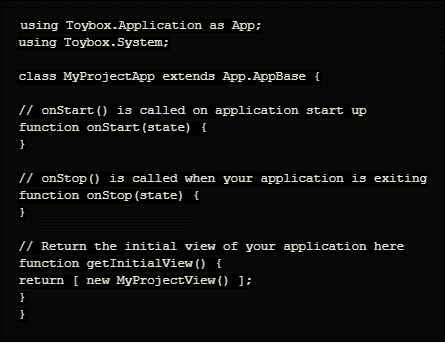
\includegraphics{images/code_snippet}
	\\
	\caption{ukázka jednoduchého fragmentu kódu v MonkeyC}
	\label{img:monkeyC_Fragment}
\end{figure}

\subsection{Monkey C a ostatní jazyky}
Stejně jako italština a španělština vznikly z latiny, Monkey C čerpá spostu věcí převážně z jiných moderních jazyků. C, Java, JavaScript, Python, Lua, Ruby a PHP, všechny tyto jazyky ovlivnily výslednou podobu Monkey C. \cite{monkeyc_2021} \\
Mezi Monkey C a výše uvedenýmy jazyky jsou přesto jisté rozdíly, které budou popsány v následujících řádcích.
\begin{enumerate}
\item \textbf{Java} - Stejně, jako Java, je Monkey C kompilování do byte kódu, který je následně interpretován virtuálním strojem. Jak už bylo zmíněno výše, virtuální stroj pro Monkey C nese název Monkey Brains. Další společná vlastnost s Javou je ta, že k alokaci objektů dochází na haldě (heap). V neposledí řadě stojí za zmínku, že virtuální stroj má na starosti čištění paměti, přičemž v Javě je toto realizováno prostřednictvím tzv. "garbage collectoru" a v Monkey C pomocí "reference countingu".
\item \textbf{JavaScript} - Hlavním rozdílem mezi mezi JavaScriptem a Monkey C spočívá v tom, že funkce v Money C nedisponují vlastností "funkce první třídy" (first-class function). "To znamená, že jazyk podporuje předávání funkcí jako argumentů jiným funkcím, jejich vrácení jako hodnoty z jiných funkcí a jejich přiřazení k proměnným nebo jejich uložení v datových strukturách." \cite{abelson1996structure}\\ Na obrázku \ref{img:callback_error} lze vidět, že při pokusu předat funkci, jako parametr jinou funkci, rozšíření detekuje operaci, která je v rozporu s Monkey C gramatikou, a tím pádem oznámí uživateli chybu.
\item \textbf{Python} - Objekty v Pythonu jsou reprezentovány, jako hashovací tabulky, přičemž funkce a proměnné lze objektům přiřazovat za běhu programu. Objekty v Monkey C jsou kompilovány ještě před spuštěním programu, a tím pádem nemohou být modifikovány za běhu. Všechny proměnné, předtím než je použijeme např. ve funkci, třídní instanci či rodičovském modulu, musí být deklarovány.
\end{enumerate}

\begin{figure}[h!]
	\centering
	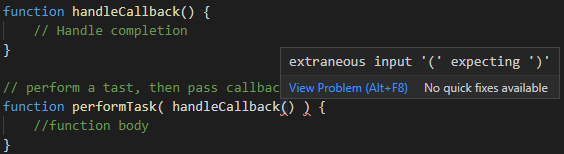
\includegraphics{images/callback_error}
	\\
	\caption{rozšíření při pokusu předat funkci, jako parametr, detekuje chybu.}
	\label{img:callback_error}
\end{figure}

\endinput